

\chapter{RNA štruktúra}
V tejto práci sa venujeme automatickej predikcii priestorovej štruktúry ribonukleovej kyseliny, 
preto sa budeme v prvej kapitole zaoberať jej významom z biologického hľadiska. 
Ďalej preberieme možnosti, akým spôsobom a aké podrobné informácie o štruktúre RNA dokáže súčasná veda získať experimentálnym spôsobom a aká je motivácia pre počítačovú predikciu RNA.   
Nakoniec uvedieme možnosti, ako RNA štruktúru reprezentovať vo formáte textových súborov a aké informácie o štruktúre jednotlivé typy súborov uchovávajú. 

\section{RNA}
Ribonukleová kyselina slúži na prenos alebo uchovávanie genetickej informácie vo všetkých živých organizmoch. Najznámejšia je jej úloha v Centrálnej dogme molekulárnej biológie \cite{Crick70}, kde slúži pri syntéze proteínov z DNA na prenášanie genetickej informácie.


\indent RNA je rovnako ako DNA tvorená štyrmi typmi nukleotidov (báz). Sú to adenín (A), guanín (G), cytozín (C) a uracil (U).  Narozdiel od RNA sa v DNA namiesto uracilu vyskytuje báza tymín (T). Jednotlivé nukleotidy sú chemicky naviazané na cukor - ribózu, ktorý ich spája do vlákna (v prípade DNA sa jedná o deoxyribózu).
Dĺžka vlákna môže byť v závislosti na type RNA od niekoľkých jednotiek až po tisíce nukleotidov. Pre DNA následne platí, že sa vodíkovými väzbami spájajú dva komplementárne reťazce do špirály, čo čiastočne určuje pravidelný tvar molekuly v priestore. RNA sa však vyskytuje hlavne v  jednovláknovej forme, pričom sa vlákno spája vodíkovými väzbami samo so sebou, a to na rôznych miestach, čo prináša veľkú variabilitu v tvare molekuly. Platí, že tromi vodíkovými väzbami sa navájom viažu nukleotidy cytozín a guanín, a dvomi väzbami nukleotidy adenín a uracil (prípadne tymín v DNA).
%\begin{figure}[p]\centering
%\includegraphics{../img/dna_6ijv}
%\caption{Príklad štruktúry molekuly DNA.}
%\label{obr01:DNA}
%\end{figure}

\section{Druhy a funkcie RNA}
Okrem prenosu genetickej informácie pri syntéze proteínov, ktorý pozostáva z replikácie DNA, transkripcie DNA do RNA a nakoniec translácie z RNA do samotnej primárnej štruktúry proteínu (pričom sa využívajú rôzne typy RNA), zastáva RNA aj iné funkcie. Slúži napríklad na uchovávanie genetickej informácie niektorých jednoduchých organizmov ako sú vírusy. Tie môžu na uchovanie genetickej informácie používať jednovláknovú RNA, dvojvláknovú RNA a v prípade retrovírusov špeciálny typ RNA, ktorý je schopný prepisovať genetickú informáciu z RNA do DNA procesom reverznej transkriptázy a vložiť tak svoju genetickú informáciu do genomu napadnutej bunky. Medzi tieto vírusy patrí napríklad známy vírus HIV.  \cite{Krupovice18}


\indent Prehľad niektorých typov RNA:
\begin{itemize}
\item kódujúca (2\%)
\begin{itemize}
\item mediátorová RNA (mRNA)
\end{itemize}
\item nekódujúca (98\%)
\begin{itemize}
\item ribozomálna RNA (rRNA)
\item prenosová RNA (tRNA)
\item funkcionálna RNA (fRNA)
\item mikro RNA (miRNA)
\item malá interferujúca (small interfering) RNA (siRNA)
\item jadrová (nuclear) RNA (snRNA)
\item jadierková (nucleolar) RNA (snoRNA)
\item vírusová RNA (vRNA)
\item dlhá nekódujúca RNA (lncRNA)
\item ďalšie...
\end{itemize}
\end{itemize}

\indent Messenger RNA (mRNA) vzniká pri prepise (transkripcii) DNA v jadre bunky. Najprv je vytvorená pre-mRNA, ktorá obsahuje aj nekódujúce úseky. V ďalšom kroku sa z nej ešte v jadre bunky procesom nazývanzým splicing odstránia intróny (nekódujúce úseky) za pomoci snRNA. snRNA rozpoznáva sekvenciu báz AGGU označujúcu prechod medzi intrónom  a exónom. Následne mRNA putuje cez póry v jadrovej membráne von do cytoplazmy, kde sa naviaže na ribozóm. \cite{Alberts02}


\indent Ribozóm obsahuje ribozomálnu RNA (rRNA), ktorá sa zúčastňuje translácie (prekladu) mRNA do primárnej skevencie kódovanej bielkoviny. Okrem toho je to typicky najčastejšie sa vyskytujúca RNA v bunke, pričom jej dĺžka môže byť až niekoľko tisíc nukleotidov.


\indent Prenosová tRNA sa nachádza v cytoplazme bunky a jej funkcia spočíva v dopravení správnej aminokyseliny do procesu translácie. Každá aminokyselina má svojú vlastnú špecifickú tRNA, na ktorú je naviazaná aminoacyl-tRNA syntetázou, a následne dopravená na miesto syntézy.


\indent  Niektoré typy RNA plnia regulačnú funkciu. Napríklad mikro RNA (miRNA) zabraňuje procesu translácie mRNA tým, že sa na ňu naviaže a zabráni jej spojeniu s ribozómom. snoRNA zas hrá úlohu pri modifikácii ostatných typov RNA - hlavne rRNA, tRNA a snRNA.


\indent Sekvencie lncRNA mávajú typicky dĺžku okolo 200 nukleotidov a jeden zo známych zástupcov je gén XIST, ktorý sa uplatňuje pri procese inaktivácie chromozómu X. \cite{Rinn a Chang, 2012}


\section{Reprezentácia a práca s RNA}
Fyzicky je RNA v bunke vlastne len mnoho atómov vodíka, kyslíka, uhlíka, dusíka a fosforu usporiadaných v priestore vďaka chemickým a fyzikálnym interakciám a vlastnostiam atómov. Pre to, aby sme ich mohli spracovávať pomocou počítača, potrebujeme vhodnú reprezentáciu štruktúry.
Typ reprezentácie závisí od toho, aké informácie o štruktúre chceme mať k dispozícii a takisto aké informácie sme schopní získať. Principiálne môžeme rozdeliť reprezentáciu RNA štruktúr na nasledujúce štyri úrovne:


\begin{itemize}
\item Primárna
\item Sekundárna
\item Terciárna
\item Kvartérna
\end{itemize}


\indent Primárna štruktúra je najviac zjednodušená reprezentácia RNA. Určuje len poradie a typ jednotlivých nukleotidov v RNA štruktúre a ďalej ju budeme v práci tiež označovať ako sekvenciu. V počítači ju reprezentujeme ako textový súbor typu fasta, ktorý má na prvom riadku identifikáciu štruktúry (názov, chain) a v ďalších riadkoch sú to len písmena A, G, C, U určujúce presné poradie nukleotidov. V prípade, že typ nukleotidu na niektorej pozícií je neznámy používame písmeno X alebo N. Primárna sekvencia RNA takisto slúži ako jeden zo vstupov pre náš prediktor a definuje sekvenciu štruktúry, ktorú cheme získať.


\indent Sekundárna štruktúra zachytáva vodíkové väzby medzi jednotlivými nukleotidmi vo vlákne RNA. Dva nukleoidy, ktoré sú spojené vodíkovou väzbou označujeme ako base pair. Vďaka spájaniu jednotlivých nukleotidov vieme v sekundárnej štruktúre pozorovať rôzne podštruktúry, ako napríklad helix, loop, pseudoknot, hairpin loop, internal loop, branch loop , stem a ďalšie \ref{obr01:secstru}. Sekundárnu štruktúru budeme v tejto práci používať na pomoc pri predikcii terciárnej štruktúry, nakoľko nám dáva informáciu o nukleotidoch, ktoré sú spojené vodíkovou väzbou a teda sa nachádzajú blízko pri sebe. Sekundárnu štruktúru molekuly budeme reprezentovať ako textový súbor, kde bodka značí, že na nukleotid danej pozícii nie je spárovaný žiadnou väzbou,base pair spojený vodíkovou väzbou je značený ako valídne uzátvorkovanie jednoduchými zátvorkami a pseudoknot býva reprezentovaný hranatými zátvorkami.  


\begin{figure}%[p]\centering
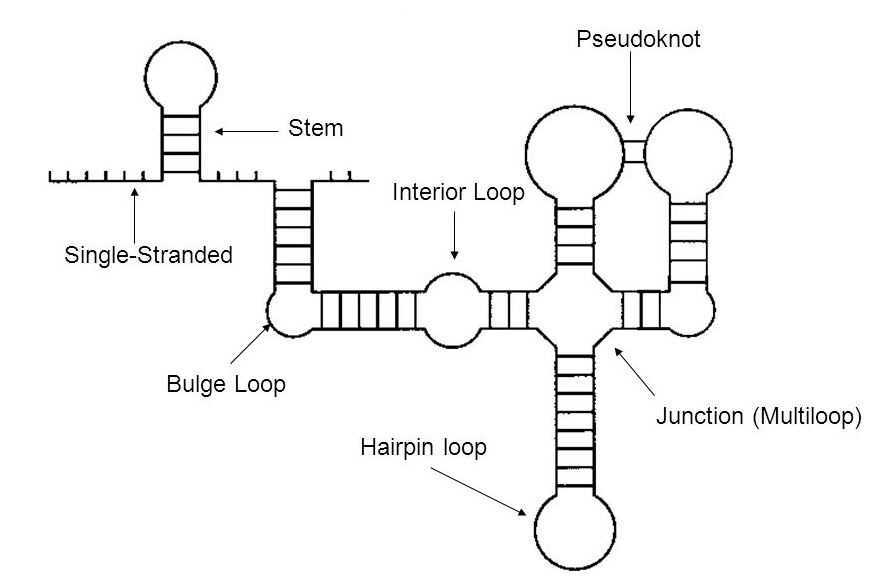
\includegraphics[width=\textwidth]{../img/secondary_structure}
\caption{Príklad nakreslenia sekundárnej štruktúre RNA. \cite{Eddy04}}
\label{obr01:secstru}
\end{figure}


\indent Zmyslom terciárnej štruktúry je popísať presné rozloženie jednotlivých atómov v trojdimenzionálnom priestore za pomoci koordinátov. V našej práci je hlavným cieľom tieto koordináty určiť za predpokladu znalosti primárnej sekvencie a terciárnych štruktúr ďalších RNA molekúl, ktoré sa pokúšame pri predikcii použiť ako vzory. 


\indent Kvarciárna štruktúra RNA popisuje vzťahy medzi celými molekulami RNA -
napríklad interakcie medzi jednotlivými molekulami RNA v ribozómoch \cite{Noller84} a taktiež vzťahy medzi RNA a molekulami bielkovín.

\section{Význam a získavanie terciárnej štruktúry}
Štruktúra RNA priamo súvisí s funkciou, ktorú vykonáva.Tvar štruktúry \ref{obr02:ecoli} určuje, ktoré enzýmy sa na ňu dokážu pripájanať a prípadne ju modifikovať a s ktorými bielkovinami a nukleovými kyselinami sa dokáže viazať. Bolo preukázané, že váčšina časti RNA štruktúry, ktoré sú schopné sa viazať s inými molekulami nie sú súčasťou žiadneho base pair-u a teda sú v sekundárnej štruktúre označené ako nespárované \cite{Schudoma10}. Zmena
terciárnej štruktúry, ktorá vedie ku strate pôvodnej funkcie molekuly, sa nazýva denaturácia.

%daj tu obrázok
\begin{figure}%[p]\centering
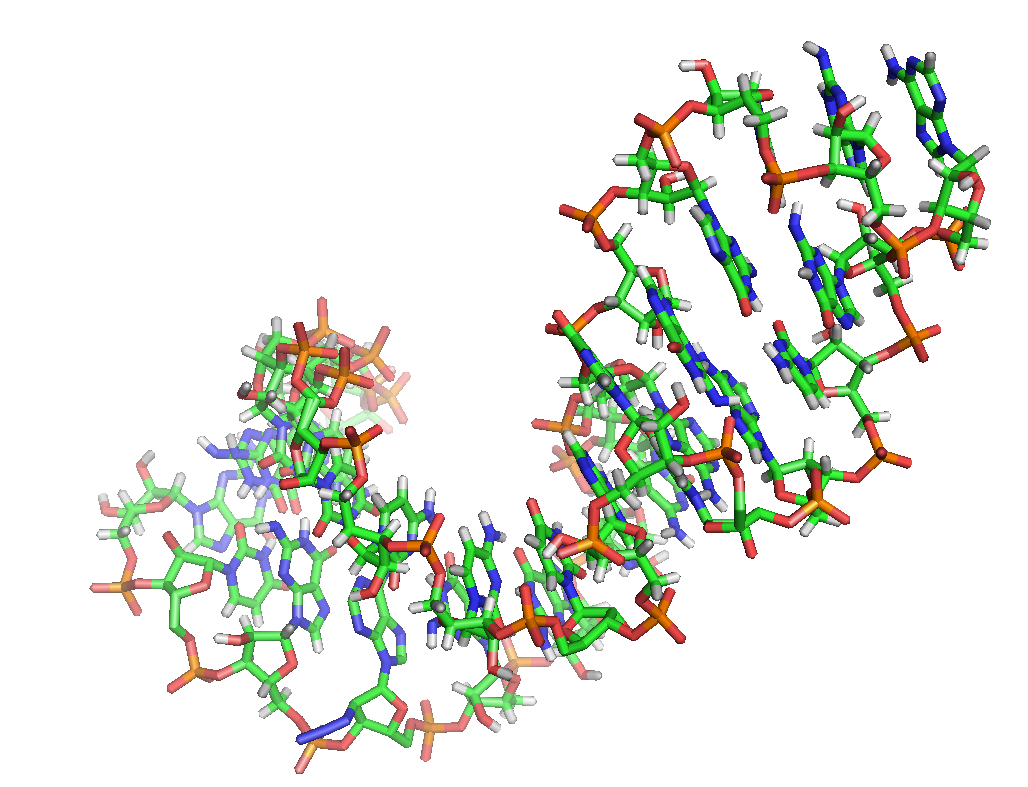
\includegraphics[width=\textwidth]{../img/ecoli_rna_example}
\caption{Príklad terciárnej štruktúry RNA nacházajúcej sa v baktérii  escherichia coli.}
\label{obr02:ecoli}
\end{figure}



\indent 
Bolo vyvinutých viacero experimentálnych metód, pomocou ktorých môžeme získať terciárnu štruktúru RNA \cite{Felden07}:
\begin{itemize}
\item metódy s vysokou presnosťou
\begin{itemize}
\item X-ray crystallography
\item Cryo-electron microscopy 
\item Nuclear Magnetic Resonance (NMR) spectroscopy
\end{itemize}
\item metódy s nižšou presnosťou
\begin{itemize}
\item Mass spectrometry
\item Chemical probing
\item Thermal denaturation
\item RNA engineering
\end{itemize}
\end{itemize}


\indent X-ray crystallography (rentgenova kryštalografia) funguje principiálne tak, že sa molekula najprv zkryštalyzuje a následne sa nasvieti rentgenovým lúčom. Z kryštálu je lúč odrazený a pritom rozdelený na viacero lúčov. Zmeraním týchto uhlova intenzity odrazených lúčov je následne možné určiť pozície jednotlivých atómov v molekule. Momentálne je to jesna z najpoužívanejších metód na získanie mnohých makromolekulárnych štruktúr. Rozlíšenie získanej štruktúry sa pohybuje okolo 2.0 Å. \ref{obr03:x-ray}


\begin{figure}%[p]\centering
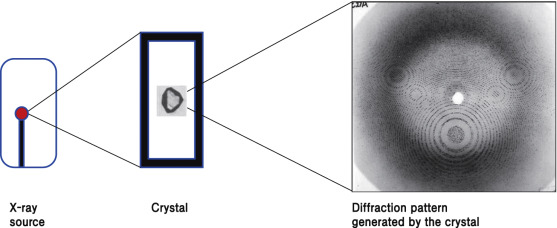
\includegraphics[width=\textwidth]{../img/x-ray}
\caption{Princíp rentgenovej kryštalografie. \cite{Ryu17}}
\label{obr03:x-ray}
\end{figure}


\indent Cryo-electron microscopy metóda využíva zmrazenie molekuly v substancií, ktorá je následne pozorovaná elektrónovým mikroskopom. Princíp metódy je známy približne od roku 1970, ale až donedávna pomocou nej nebolo možné získať tak presné vysledky, ako pomocou rentgenovej kryštalografie. Na druhej strane dĺžka skúmanej štruktúry nie je pri tejto metóde tak limitujúcim faktorom. V roku 2017 bola udelená nobelová cena za chémiu  J. Dubochetovi, J. Frankovi a  R. Hendersonovi za vyvinutie metódy, ktorou sa dá získať atómová štruktúra molekuly s vysokým rozlíšením.


\indent Metóda Nuclear Magnetic Resonance je založená na pôsobení statického magnetického poľa na jadrá atómov v molekule. Je vhodná hlavne na získavanie kratších štruktúr.


\indent Experimentálne prístupy sa od seba navzájom líšia presnosťou výsledku, dĺžkou štruktúry s ktorou sú schopné pracovať, ale ich hlavnám problémom je, že sú stále časovo náročné a drahé. Pretože získanie primárnej štruktúry RNA a proteinov je oveľa ľahšia úloha, začali byť skúmané aj možnosti, ako predikovať sekundárnu a terciárnu štruktúru za pomoci počítača, čomu sa budeme v našej práci venovať.